%%%%%%%%%%%%%%%%%%%%%%%%%%%%%%%%%%%%%%%%%
% Document Author: Plinio H. Vargas
% Course: CS-532, Spring 2016 at Old Dominion University
%
% Structured General Purpose Assignment
% LaTeX Template
%
% This template has been downloaded from:
% http://www.latextemplates.com
%
% Original template author:
% Ted Pavlic (http://www.tedpavlic.com)
%
% Note:
% The \lipsum[#] commands throughout this template generate dummy text
% to fill the template out. These commands should all be removed when 
% writing assignment content.
%
%%%%%%%%%%%%%%%%%%%%%%%%%%%%%%%%%%%%%%%%%
%----------------------------------------------------------------------------------------
%	PACKAGES AND OTHER DOCUMENT CONFIGURATIONS
%----------------------------------------------------------------------------------------

\documentclass{article}

\usepackage{fancyhdr} % Required for custom headers
\usepackage{lastpage} % Required to determine the last page for the footer
\usepackage{extramarks} % Required for headers and footers
\usepackage{listings}
\usepackage{graphicx} % Required to insert images
\usepackage{lipsum} % Used for inserting dummy 'Lorem ipsum' text into the template
\usepackage[bookmarks,bookmarksopen,bookmarksdepth=2]{hyperref} % for bookmarks
\usepackage{enumerate}
\usepackage{csquotes} % for quoting things
\usepackage{multirow}
\usepackage{amsmath}
\usepackage{caption}
\usepackage{navigator}%\usepackage{caption}
\usepackage[shortlabels]{enumitem}
\usepackage{enumitem}
\usepackage{lmodern}
\usepackage[utf8]{inputenc}
%\usepackage[table]{xcolor}% http://ctan.org/pkg/xcolo
\usepackage[dvipsnames]{xcolor}
\usepackage{longtable}
\usepackage{textcomp}
\usepackage{url}
\usepackage{import}
\usepackage{float}
\usepackage{dashrule} % for dashline
\usepackage{keystroke}
\usepackage{amssymb}

\lstdefinestyle{numbers}
{ frame=tb,
  language=python,
  aboveskip=3mm,
  belowskip=3mm,
  showstringspaces=false,
  columns=flexible,
  basicstyle={\small\ttfamily},
  numbers=left,
  numberstyle=\tiny\color{gray},
  keywordstyle=\color{blue},
  commentstyle=\color{OliveGreen},
  stringstyle=\color{purple},
  breaklines=true,
  breakatwhitespace=true,
  tabsize=3
}

\lstdefinestyle{nonumbers}
{ frame=shadowbox,
  language=python,
  aboveskip=3mm,
  belowskip=3mm,
  showstringspaces=false,
  columns=flexible,
  basicstyle={\small\ttfamily},
  numbers=none,
  numberstyle=\tiny\color{gray},
  keywordstyle=\color{blue},
  commentstyle=\color{OliveGreen},
  stringstyle=\color{purple},
  breaklines=true,
  breakatwhitespace=true,
  tabsize=3
}

\lstdefinestyle{mybox}
{
	basicstyle={\small\ttfamily},
    numbers=left,
    numberstyle=\tiny\color{gray},
    stepnumber=1,
    numbersep=5pt,
    showspaces=false, % don't show spaces by adding underscores
    showstringspaces=false, % don't underline spaces in strings
    showtabs=false, % don't show tabs with underscores
    frame=shadowbox,
    tabsize=4,
    captionpos=b,
    breaklines=true,
    breakatwhitespace=false,
  	keywordstyle=\color{blue},
	commentstyle=\color{OliveGreen},
  	stringstyle=\color{purple},    
    rulesepcolor=\color{red!20!green!20!blue!20},
    numberbychapter=false,
    stringstyle=\color{purple},
}


\providecommand{\providehyphenmins}[2]{}

% Margins
\topmargin=-0.45in
\evensidemargin=0in
\oddsidemargin=0in
\textwidth=6.5in
\textheight=9.0in
\headsep=0.25in 

\linespread{1.1} % Line spacing
\newcommand*{\medtau}{\mathbin{\scalebox{1.5}{$\tau$}}}% increase size of tau
\newcommand*{\medtaub}{\mathbin{\scalebox{1.5}{$\tau_b$}}}% increase size of tau_b
\newcommand\multibrace[3]{\rdelim\}{#1}{3mm}[\pbox{#2}{#3}]}

% Set up the header and footer
\pagestyle{fancy}
\lhead{\hmwkAuthorName} % Top left header
\chead{\hmwkShortClass\ (\hmwkClassInstructor\ \hmwkClassTime): \hmwkShortTitle} % Top center header
%\rhead{\firstxmark} % Top right header
\rhead{} % Top right header
\lfoot{\lastxmark} % Bottom left footer
\cfoot{} % Bottom center footer
\rfoot{Page\ \thepage\ of\ \pageref{LastPage}} % Bottom right footer
\renewcommand\headrulewidth{0.4pt} % Size of the header rule
\renewcommand\footrulewidth{0.4pt} % Size of the footer rule

\setlength\parindent{0pt} % Removes all indentation from paragraphs

%----------------------------------------------------------------------------------------
%	DOCUMENT STRUCTURE COMMANDS
%	Skip this unless you know what you're doing
%----------------------------------------------------------------------------------------

% Header and footer for when a page split occurs within a problem environment
\newcommand{\enterProblemHeader}[1]{
\nobreak\extramarks{#1}{#1 continued on next page\ldots}\nobreak
\nobreak\extramarks{#1 (continued)}{#1 continued on next page\ldots}\nobreak
}

% Header and footer for when a page split occurs between problem environments
\newcommand{\exitProblemHeader}[1]{
\nobreak\extramarks{#1 (continued)}{#1 continued on next page\ldots}\nobreak
\nobreak\extramarks{#1}{}\nobreak
}

\newcounter{sub}[section]
\newenvironment{sub}[1][]{\stepcounter{sub}\thesub #1}{ }

\setcounter{secnumdepth}{0} % Removes default section numbers
\newcounter{homeworkProblemCounter} % Creates a counter to keep track of the number of problems
\newcommand{\sectionNumber}{\arabic{homeworkProblemCounter}.\sub }


\newcommand{\homeworkProblemName}{}
\newenvironment{homeworkProblem}[1][Problem \arabic{homeworkProblemCounter}]{ % Makes a new environment called homeworkProblem which takes 1 argument (custom name) but the default is "Problem #"
\stepcounter{homeworkProblemCounter} % Increase counter for number of problems
\setcounter{sub}{0}
\renewcommand{\homeworkProblemName}{#1} % Assign \homeworkProblemName the name of the problem
\
\section{\homeworkProblemName} % Make a section in the document with the custom problem count
\enterProblemHeader{\homeworkProblemName} % Header and footer within the environment
}{
\exitProblemHeader{\homeworkProblemName} % Header and footer after the environment
}

\newcommand{\problemAnswer}[1]{ % Defines the problem answer command with the content as the only argument
\noindent\framebox[\columnwidth][c]{\begin{minipage}{0.98\columnwidth}#1\end{minipage}} % Makes the box around the problem answer and puts the content inside
}

\newcommand{\homeworkSectionName}{}
\newenvironment{homeworkSection}[1]{ % New environment for sections within homework problems, takes 1 argument - the name of the section
\renewcommand{\homeworkSectionName}{#1} % Assign \homeworkSectionName to the name of the section from the environment argument
\subsection{\homeworkSectionName} % Make a subsection with the custom name of the subsection
\enterProblemHeader{\homeworkProblemName\ [\homeworkSectionName]} % Header and footer within the environment
}{
\enterProblemHeader{\homeworkProblemName} % Header and footer after the environment
}
   
%----------------------------------------------------------------------------------------
%	NAME AND CLASS SECTION
%----------------------------------------------------------------------------------------

\newcommand{\hmwkTitle}{\\Assignment\ \#10: \\kNN and SVM} % Assignment title
\newcommand{\hmwkShortTitle}{Assignment 10} % Assignment title
\newcommand{\hmwkDueDate}{Saturday,\ April 30,\ 2016} % Due date
\newcommand{\hmwkClass}{CS-432/532 Introduction to Web Science} % Course/class
\newcommand{\hmwkShortClass}{CS-432/532 Web Science} % Course/class
\newcommand{\hmwkClassTime}{- Spring 2016} % Class/lecture time
\newcommand{\hmwkClassInstructor}{Dr.  Michael L. Nelson} % Teacher/lecturer
\newcommand{\hmwkAuthorName}{Plinio Vargas} % Your name
\newcommand{\hmwkAuthorEmail}{pvargas@cs.odu.edu} % Your name
%------------------------------------------------------------
% Algorithm declaration
%------------------------------------------------------------
\lstnewenvironment{algorithm}[1][] %defines the algorithm listing environment
{   
    %\refstepcounter{nalg} %increments algorithm number
    \captionsetup{labelsep=colon} %defines the caption setup for: it ises label format as the declared caption label above and makes label and caption text to be separated by a ':'
    \lstset{ %this is the stype
        frame=tB,
        numbers=left, 
        mathescape=true,
        numberstyle=\tiny,
        basicstyle={\small\ttfamily}, 
        keywordstyle=\color{blue}\bfseries\em,
        keywords={,input, output, return, 
                   datatype, function, in, 
                   if, else, for, foreach, 
                   while, write, begin, end, 
        } %add the keywords you want, or load a language as Rubens explains in his comment above.
        numbers=left,
        xleftmargin=.04\textwidth,
        #1 % this is to add specific settings to an usage of this environment (for instnce, the caption and referable label)
    }
}
{}
%----------------------------------------------------------------------------------------
%	TITLE PAGE
%----------------------------------------------------------------------------------------

\title{
\vspace{2in}
\textmd{\textbf{\hmwkClass:\ \hmwkTitle}}\\
\normalsize\vspace{0.1in}\small{Due\ on\ \hmwkDueDate}\\
\vspace{0.1in}\large{\textit{\hmwkClassInstructor\ }}
\vspace{3in}
}

\author{\textbf{\hmwkAuthorName} \\ \hmwkAuthorEmail}
\date{} % Insert date here if you want it to appear below your name

%----------------------------------------------------------------------------------------
%	EMBEDDED FILE
%----------------------------------------------------------------------------------------
%\embeddedfile{KarateClub}{../KarateClub.py}
%\embeddedfile{DrawOriginalClub}{../DrawOriginalClub.py}
%----------------------------------------------------------------------------------------
%	START OF DOCUMENT
%----------------------------------------------------------------------------------------
\begin{document}

\clearpage\maketitle
\thispagestyle{empty}

%----------------------------------------------------------------------------------------
%	TABLE OF CONTENTS
%----------------------------------------------------------------------------------------

%\setcounter{tocdepth}{1} % Uncomment this line if you don't want subsections listed in the ToC

\newpage
\clearpage\tableofcontents
\listoffigures
\lstlistoflistings
\listoftables

\thispagestyle{empty}
\newpage
\setcounter{page}{1}
%----------------------------------------------------------------------------------------
%	Problem 1
%----------------------------------------------------------------------------------------
\begin{homeworkProblem}% Custom section title
\vspace*{10pt} % Question
Using the data from A8:
\begin{itemize}
\item Consider each row in the blog-term matrix as a 500 dimension vector, 
corresponding to a blog. 

\item From chapter 8, replace numpredict.euclidean() with cosine as the 
distance metric.  In other words, you'll be computing the cosine between
vectors of 500 dimensions.  

\item Use knnestimate() to compute the nearest neighbors for both:

\end{itemize}

\url{http://f-measure.blogspot.com/}\\
\url{http://ws-dl.blogspot.com/}\\

for k=\{1,2,5,10,20\}.
\subsection{1.1 Approach}
In order to complete this problem, three modules from \cite{ci} were taken and modified: \textbf{knnestimate}, \textbf{getdistances} and \textit{euclidean}, the latest changed to \textbf{cosine\_distance}. The heart of this approach resides in the \textbf{cosine\_distance} module (see Listing \ref{lst:calculator}), which takes as a parameter two 500-dimensional vectors.\\

\lstinputlisting[language=python,
                 style=mybox, 
                 captionpos=t,
                 caption={Cosine Calculator: CosineDistance.py},
                 label={lst:calculator},
				 linerange={65-70},
				 firstnumber=65            
                 ]
{../CosineDistance.py}
\vspace{5mm}
Since $\cos \theta$ for any point is equal to 1 when $x$ and $y$ are equal in our plotting coordinate, if the cosine distance calculation between vector $v_1$ and $v_2$ is equal to zero, then  $v_1$ = $v_2$. The further from 0 the calculation between $v_1$ and $v_2$ is,  the greater the difference is between them.\\

Using the same approach as in \cite{ci}, the values are loaded into a dictionary object (\textbf{data}). Term values are  extracted from the first line of the input file (see Listing \ref{lst:main} line 21).\\



\lstinputlisting[language=python,
                 style=mybox, 
                 captionpos=t,
                 caption={Main Module: CosineDistance.py},
                 label={lst:main},
				 linerange={9-46},
				 firstnumber=9           
                 ]
{../CosineDistance.py}
\vspace{5mm}
The blog's title (line 24) is obtained  by removing the 500-dimensional vector values  from the file entry row. To obtain the row index  from our two studied blogs, we visually inspected the entry file (\textit{blogdata.tx}). Index \textcolor{blue}{76} corresponded to \url{http://f-measure.blogspot.com/}; index \textcolor{blue}{68} corresponded to \url{http://ws-dl.blogspot.com/}\\

In order to get the cosine-distance between two blogs, we passed the vector values to function \textit{getdistances}. As the textbook explains, it \enquote{calls the distance function on the vector given against every other vector in the dataset and puts them in a big list. The list is sorted so that the closest item is on the top}.

\lstinputlisting[language=python,
                 style=mybox, 
                 captionpos=t,
                 caption={Getdistances Module: CosineDistance.py},
                 label={lst:getdistances},
				 linerange={49-62},         
                 ]
{../CosineDistance.py}

\vspace{10mm}
To display k-blogs closest to blog-$x$, an iteration is performed to call function \textit{knnestimate}. This function, a modification from \cite{ci}, simply returns the k-elements from the sorted list provided by function \textit{getdistances} between blog-$x$ and the other 99 blogs.\\

\lstinputlisting[language=python,
                 style=mybox, 
                 captionpos=t,
                 caption={Knnestimate Module: CosineDistance.py},
                 label={lst:knnestimate},
				 linerange={73-84},         
                 ]
{../CosineDistance.py}

\newpage
\subsection{1.2 Solution}
Since we clustered our 100 blogs in assignment 8, we can use the previous work as a comparison. Tables 1 through 10 contain our two blog similarities among the selected 100 blogs, using  cosine-distance calculator.  \\

According to Table \ref{tab:fm-k1}, the most similar blog to \textbf{F-Measure} is \url{http://didnotchart.blogspot.com/}. This blog passed the eye test since it is also a blog related to music. Looking at the dendrogram from assignment 8, \enquote{Did Not Chart} is clustered close to \textbf{F-Measure}, but is not the closest. \textbf{F-Measure} was clustered closer to \url{http://ihatethe90s.blogspot.com/}. The last is also a blog related to music, so it also passed the eye test.\\

Then, which blog is the most similar to \textbf{F-Measure}? \url{http://ihatethe90s.blogspot.com/} or \url{http://didnotchart.blogspot.com/}? To answer this question we need to dive into the raw data, the DNA of our research:\\

DidNotChart\\
2011058000030020120100000000132022016002000110710140230401110000213323100000002822\\
1102104201470307210000271830001010130110000007300240105000000011301301112000042010\\
0061105200020020011006000050060012000101002110210320314001000004000110100002206011\\
0090010110300003131003420100000400620901001000008201031120110100014103030105538042\\
0301011000000110301120411100000023000020003000102000001360000110300410041200317001\\
1010512002001800001051150110310310001001000074007125001021300200403010010101050110\\
110330000000110000\\

F-Measure\\
2001000380111111362100040000010001013000000109010200210000010004000012032000200251\\
0000010041090502001010081260312211022400100302040005030110005101020020200212124040\\
2111214480000200001220800011001001110000101020210183022020103001101234020021821031\\
0120051016004100020030201000001010300011240012000110161011002200200114600000212222\\
0221002031422000150202025030330110000505100001110020000100100015000602000014140101\\
0130600118007100010001600110001080110200000012142000005001025003016010101140030101\\
20500130200212330060\\

IHateThe90s\\
5410143611006300011153261001450341014154144103110204150232112250740402910902119131\\
1274001966276235740638572282415100014910212011827014312221667521601610020114504224\\
3503713405016477401112118800214131713025333403030220527161217310458621330327411261\\
2339112264622111360142121313225128312673441211131110146111120093036121633230260135\\
5224414116022175331910320211641030125491745601965317211133914122066001526116214130\\
3116232430346315842341237301310760156050201822631080330161565567576122811132101343\\
0434176111324110139300122076451710610601512052912135803628211270000001121511821215\\
216531111147034\\

To understand the raw data above, we need to inspect the 500 matrix file: \textit{blogdata.txt}. The DNA thickness difference between I-Hate-The-90s and F-Measure is not due to extra terms, but rather many term frequency in I-Hate-The-90s. The differences are in the double digits, while in F-Measure and Did-Not-Chart, the differences are in the single digits. Then, although the blogs could be talking about the same thing, their frequencies are so far apart that they make them less similar.\\

As we expand the number of blog k-neighbors for K=20, an examination to the most distant neighbors \enquote{funky little demons} revealed this blog is not exactly about music, but it has lyrics which are related to music. Looking at dendrogram from assignment 8, \enquote{funky little demons} was not clustered near \textbf{F-Measure}, and the deepest element in the cluster is \url{http://kidchair.blogspot.com/}, which is about songs (music).\\

F-Measure\\
2001000380111111362100040000010001013000000109010200210000010004000012032000200251\\
0000010041090502001010081260312211022400100302040005030110005101020020200212124040\\
2111214480000200001220800011001001110000101020210183022020103001101234020021821031\\
0120051016004100020030201000001010300011240012000110161011002200200114600000212222\\
0221002031422000150202025030330110000505100001110020000100100015000602000014140101\\
0130600118007100010001600110001080110200000012142000005001025003016010101140030101\\
20500130200212330060\\

funkylittledemons\\
0000000200000000000000000000002000000000000000000000000000000001000000000000000000\\
0001010000000000000000000000000010000000000210000000000000000000000000000000000000\\
0000010000000000010000000000000000000000000010000100000001000000000010000000000000\\
0000000000000000001010000010000001000000000000000000000000000000000000000000000000\\
0000001000010000100000001100000100000000001001000000000000000000000000000010001000\\
0000000100030000200000100000000000000000000000000000000000010000000000000000000000\\
00000000\\

KiDCHAIR\\
1600102010030100220010000012200000001011000000111000320020022020020100330000001101\\
3000000220403080100000015230000172011000101000000500001000003300122100010015112010\\
0021024010000210600210020000120030040011000021204000000110201310000000000102010113\\
0172030000010000100010000010401002013030002110010020012000113100500000011101000001\\
0000101510021210010310300011600100000000300120001100107110000004100021120503100010\\
0004010200100001060010101000002100010002600001510201101100200000010122165101001111\\
0000101041000\\

The answer to the question which one is more similar to \textbf{F-Measure} between the last two blogs is more difficult to answer from a 40K-feet-view looking at their DNAs. The frequency of 500 terms in \enquote{funky little demons} is very low; many elements in the vector have zero values. We could be very quick to say that \url{http://kidchair.blogspot.com/} is more similar to \textbf{F-Measure}  than \enquote{funky little demons}, but if we were going element by element in the vector, we will notice the combined difference of the last blog is smaller.\\

A surprising result was the comparison with \url{http://ws-dl.blogspot.com/}. The closest blog in similarity was \url{http://lostintheshuffle899.blogspot.com/} - Lost in the Shuffle (see Table \ref{tab:wc-k1}); however in the dendrogram from assignment 8, it was clustered closer to \textbf{SpinitronBlog}. \\

Using similar comparison to their DNAs, we can notice \textbf{SpinitronBlog} does not have too many terms while \textbf{LostintheShuffle} does, making it closer by default.\\

WebScienceandDigitalLibrariesResearchGroup\\
3800605137033020145201800443102040118128020060021020010112007011207710014600000031\\
7131702030031167060300019306001230101301900040113101800001208002000010100211060413\\
3075030204511041112157802890560271238200024611100723112092600200015630000007370010\\
6843114500301131012124200206105100050201310880020190100050002000860133022000000031\\
2615000101340100010200231360210011150140004014172012242045011200011501183800022121\\
0254012010003512030003000221310206097212151313220710130201101111001792541113150270\\
00220010000006070201243010011000010019180101640004105100103130213390100050212\\

LostintheShuffle\\
0002030202200010014200121000001051001000000010021000002001010000000500010012161000\\
2102000014010100002000010011000301010000130000201000000001000000120000001012200110\\
2800210100000102000000001601000110203200001001300003100010001020100410220010102000\\
0000101000100002110000102000000300000000100000106033140001000000000002002000410000\\
0000000400001000011011017101010000000090001011190200111012121000000200010000001021\\
0001010031110100200000010400203100002030000000000000910170002200200010000002500030\\
111000000000000010\\

SpinitronBlog\\
0000000000000000000001000000000000010000000000000000000300000000001000000010005070\\
0000000000000061001000000000007000000000003000000000000000000000100000000100000000\\
0010000000000010000000000000000000000000000001000000020000100000100000000000000000\\
0000201000001000010000000000000000000000000010000000000000000000000000000000000000\\
0220100000200000010000000110019000000001000000000010000000000090000000001010010000\\
0000000050000010001100000000000000000000000000000000000000000000000005000000000300\\
00000000000\\

Blog-Terms:\\
groups-ashtray-stretching-sum-indians-adventure-rightly-cell-reviewing-tstyle-reverse-\\
statements-chilling-existent-sleepy-fortunately-typically-settle-exit-lone-behave-\\
compositions-bastards-canned-pagination-jacob-reflective-legit-eleven-exclusively-\\
spending-rival-wings-license-norm-encourage-haircut-emerge-actors-beg-honored-closet-\\
outfits-pr-collector-whore-teenagers-leisure-mob-ali-marry-hopeful-jobs-knocking-westerns-\\
pleased-females-elliot-someday-cutting-ken-historic-harris-meditation-insane-chant-myth-\\
challenge-passive-longing-curse-lenny-jewelry-ducks-supreme-joan-graduation-nigel-\\
recordings-pedal-security-tale-butter-redhead-spice-oklahoma-html-ringing-combine-army-\\
sentiments-funk-cuff-violence-orbit-producer-ariel-switched-snakes-careless-equation-arriving-\\
larger-syd-trivia-sharp-quit-critic-benefits-norton-colbert-glen-industry-clue-appeared-\\
rivers-shaking-recipe-expanded-undoubtedly-endings-dancer-sailing-viewed-jurado-drove-kil-\\
sheen-cassettes-steam-twigs-rockabilly-pummeling-reminder-sensibility-practically-lame-grande-\\
resulting-chatter-afghan-remembering-breathtaking-carl-alps-happiness-buying-carrie-careers-\\
dual-bucks-origins-quintessential-infinite-andrews-sunny-tower-chapters-ipod-immortal-ma-\\
historically-cinema-escaped-abuse-powered-eric-argue-lip-approaches-schools-cramps-ash-blogged-\\
gentleman-caring-downs-cos-appropriate-attempting-accepting-mo-eliminate-polar-cornell-flash-\\
christian-leaning-electricity-strongly-grief-polite-responsible-rebellion-fake-rides-implies-ha-\\
melvins-remove-plethora-gained-bundle-mc-crashed-astronaut-celebrate-fists-patient-knowledge-\\
pulled-wives-symphony-laundry-instinct-spiritualized-mister-allow-landed-minority-futuristic-\\
catches-surprises-claimed-index-railroad-fictional-luke-importance-aquarium-daddy-neighbors-\\
fourteen-dime-kim-sports-delay-loser-slower-kramer-gutter-grinding-pro-gods-vocabulary-movies-\\
goal-mondays-birth-mould-partnership-skinny-upcoming-grandfather-delivering-groundbreaking-\\
jacuzzi-skills-announcement-insanely-sprawling-lucas-discography-served-humming-ashley-idiots-\\
crows-truckers-subsequently-amused-effortlessly-haze-additions-flourishes-mccarthy-heath-\\
execution-formed-tons-analysis-winding-percentage-evokes-donuts-impress-outlet-zone-surviving-\\
julian-complain-wheels-palace-edward-shaped-ratio-tones-ry-cred-trapped-puppets-simpson-insert-\\
consume-zeppelin-virtue-eps-nostalgic-alaska-bend-swallowed-accidentally-hallelujah-russia-\\
directed-misery-greg-bizarre-dean-exhausting-eccentric-formerly-clicks-accurate-crashes-mod-\\
rarity-goodies-kenny-shannon-pros-categories-majority-audible-cosmic-euro-proven-product-remedy-\\
elliott-problematic-amongst-slate-blew-expert-tribe-circus-vox-iris-ny-ye-crushed-cartoon-\\
parties-university-hyper-sidewalk-jan-trials-promised-wisconsin-grape-victims-matched-graphic-\\
booker-umbrella-eternal-junior-swamp-oil-drake-originality-apartment-potter-marianne-explosive-\\
dum-lily-chromatics-magnet-disgusting-pockets-stanley-assured-oldham-illustrated-legend-ads-\\
logo-continent-noir-respond-tribal-sites-barnes-delivery-impression-health-info-chairs-los-\\
straw-directors-desk-simone-thin-cheaper-thrive-allen-maiden-elite-ab-combined-venue-jonny-\\
nothings-emergency-axis-studied-necessity-bush-confirm-newest-walker-shades-windows-realistic-\\
handy-mystic-correct-palmer-eden-sans-observed-coachella-gimmick-fashioned-traded-titus-ellis-\\
couch-bean-bursts-labor-quietly-featured-tease-species-louise-guessed-reviewer-experimental-ms-\\
overhead-breakdown-drifting-amy-finest-northwest-babes-lonesome-owls-korea-bow-swords-\\
confidence-suzanne-observations-trumpet-pile-hating-reflects-websites-horribly-cheating-sufjan-\\
intensity-advantage-engage-zombie-laced-moore-wears-tremendous-winners-songwriters-concise-\\
temptation-entering-jefferson-casey-veteran-coincidentally-distorted-riding-worlds-germans-\\
lang-manning\\



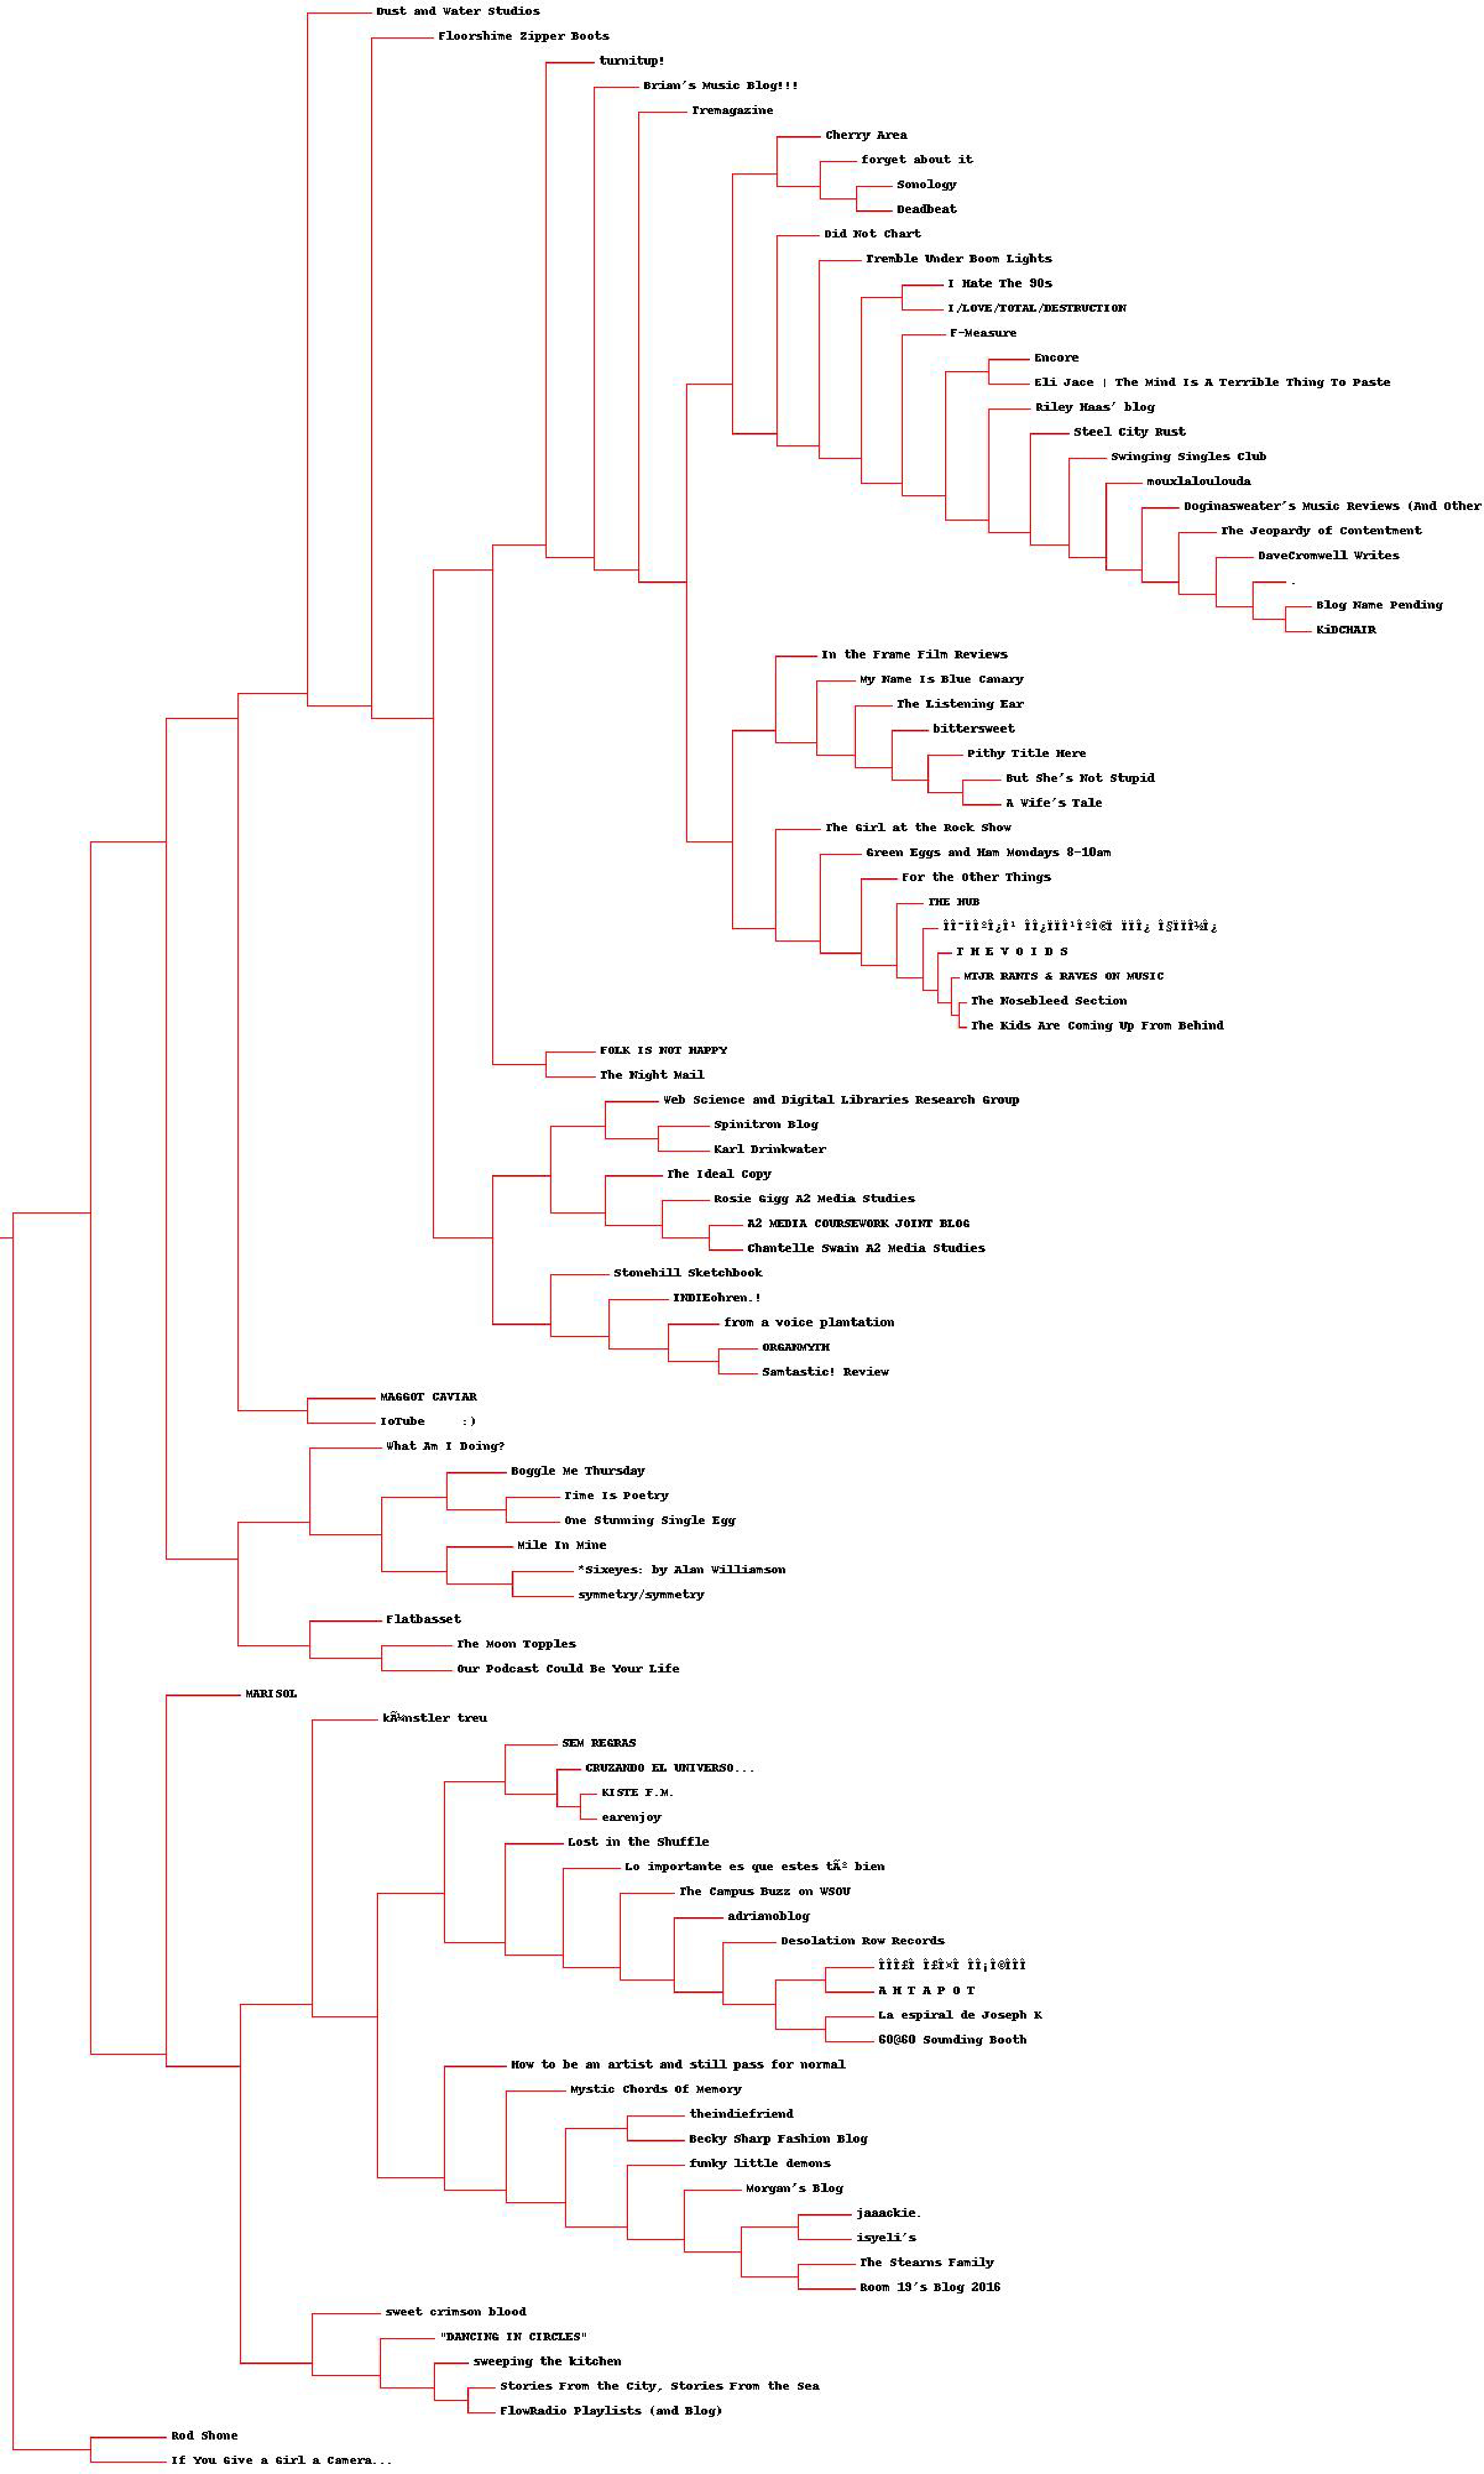
\includegraphics[scale=.3]{images/blogclust.pdf}
%----------------------------------------------------------------------------------------
%	Table F-Measure K1
%-------------------------------------------------------------------------------------
\begin{table}[!htbp]
	\caption{F-Measure with K=1} \label{tab:fm-k1}
	\begin{center}
	\vspace{-5mm}
	%\begin{minipage}{0.40\textwidth}
	\begin{tabular}{l}
		\hline
   		Blog Title\\
		\hline
		Did Not Chart\\
		\\
		\hline
	\end{tabular}
	\caption*{\scriptsize Closest K-Blogs to F-Measure for K=1.\\ Values obtained from CosineDistance.py}
	%\end{minipage}
	 \end{center}
\end{table}

%----------------------------------------------------------------------------------------
%	Table F-Measure K2
%-------------------------------------------------------------------------------------
\begin{table}[!ht]
	\caption{F-Measure with K=2} \label{tab:fm-k2}
	\begin{center}
	\vspace{-5mm}
	%\begin{minipage}{0.40\textwidth}
	\begin{tabular}{l}
		\hline
   		Blog Title\\
		\hline
		Did Not Chart\\
		THIS CHARMING YAN\\
		\\
		\hline
	\end{tabular}
	\caption*{\scriptsize Closest K-Blogs to F-Measure for K=2.\\ Values obtained from CosineDistance.py}
	%\end{minipage}
	 \end{center}
\end{table}

\newpage
%----------------------------------------------------------------------------------------
%	Table F-Measure K5
%-------------------------------------------------------------------------------------
\begin{table}[!ht]
	\caption{F-Measure with K=5} \label{tab:fm-k5}
	\begin{center}
	\vspace{-5mm}
	%\begin{minipage}{0.40\textwidth}
	\begin{tabular}{l}
		\hline
   		Blog Title\\
		\hline
		Did Not Chart\\
		THIS CHARMING YAN\\
		Encore\\
		isyeli's\\
		If You Give a Girl a Camera...		\\
		\\
		\hline
	\end{tabular}
	\caption*{\scriptsize Closest K-Blogs to F-Measure for K=5.\\ Values obtained from CosineDistance.py}
	%\end{minipage}
	 \end{center}
\end{table}

%----------------------------------------------------------------------------------------
%	Table F-Measure K10
%-------------------------------------------------------------------------------------
\begin{table}[!ht]
	\caption{F-Measure with K=10} \label{tab:fm-k10}
	\begin{center}
	\vspace{-5mm}
	%\begin{minipage}{0.40\textwidth}
	\begin{tabular}{l}
		\hline
   		Blog Title\\
		\hline
		Did Not Chart\\
		THIS CHARMING YAN\\
		Encore\\
		isyeli's\\
		If You Give a Girl a Camera...		\\
		mattgarman\\
		Rants from the Pants\\
		60@60 Sounding Booth\\
		turnitup!\\
		Doginasweater's Music Reviews (And Other ..)\\
		\\
		\hline
	\end{tabular}
	\caption*{\scriptsize Closest K-Blogs to F-Measure for K=10.\\ Values obtained from CosineDistance.py}
	%\end{minipage}
	 \end{center}
\end{table}

\newpage
%----------------------------------------------------------------------------------------
%	Table F-Measure K20
%-------------------------------------------------------------------------------------
\begin{table}[!ht]
	\caption{F-Measure with K=20} \label{tab:fm-k20}
	\begin{center}
	\vspace{-5mm}
	%\begin{minipage}{0.40\textwidth}
	\begin{tabular}{l}
		\hline
   		Blog Title\\
		\hline
		Did Not Chart\\
		THIS CHARMING YAN\\
		Encore\\
		isyeli's\\
		If You Give a Girl a Camera...		\\
		mattgarman\\
		Rants from the Pants\\
		60@60 Sounding Booth\\
		turnitup!\\
		Doginasweater's Music Reviews (And Other ..)\\
		\enquote{DANCING IN CIRCLES}\\
		I/LOVE/TOTAL/DESTRUCTION\\
		Lost in the Shuffle\\
		this time tomorrow\\
		Web Science and Digital Libraries Research Group\\
		FlowRadio Playlists (and Blog)\\
		.\\
		Stories From the City, Stories From the Sea\\
		The Jeopardy of Contentment\\
		funky little demons		\\
		\\
		\hline
	\end{tabular}
	\caption*{\scriptsize Closest K-Blogs to F-Measure for K=20.\\ Values obtained from CosineDistance.py}
	%\end{minipage}
	 \end{center}
\end{table}


%----------------------------------------------------------------------------------------
%	Table dl.blogspot.com K1
%-------------------------------------------------------------------------------------
\begin{table}[!htbp]
	\caption{dl.blogspot.com with K=1} \label{tab:wc-k1}
	\begin{center}
	\vspace{-5mm}
	%\begin{minipage}{0.40\textwidth}
	\begin{tabular}{l}
		\hline
   		Blog Title\\
		\hline
		Lost in the Shuffle\\
		\\
		\hline
	\end{tabular}
	\caption*{\scriptsize Closest K-Blogs to dl.blogspot.com for K=1.\\ Values obtained from CosineDistance.py}
	%\end{minipage}
	 \end{center}
\end{table}


%----------------------------------------------------------------------------------------
%	Table dl.blogspot.com K2
%-------------------------------------------------------------------------------------
\begin{table}[!htbp]
	\caption{dl.blogspot.com with K=2} \label{tab:wc-k2}
	\begin{center}
	\vspace{-5mm}
	%\begin{minipage}{0.40\textwidth}
	\begin{tabular}{l}
		\hline
   		Blog Title\\
		\hline
		Lost in the Shuffle\\
		\enquote{DANCING IN CIRCLES}\\
		\\
		\hline
	\end{tabular}
	\caption*{\scriptsize Closest K-Blogs to dl.blogspot.com for K=1.\\ Values obtained from CosineDistance.py}
	%\end{minipage}
	 \end{center}
\end{table}

%----------------------------------------------------------------------------------------
%	Table dl.blogspot.com K5
%-------------------------------------------------------------------------------------
\begin{table}[!htbp]
	\caption{dl.blogspot.com with K=5} \label{tab:wc-k5}
	\begin{center}
	\vspace{-5mm}
	%\begin{minipage}{0.40\textwidth}
	\begin{tabular}{l}
		\hline
   		Blog Title\\
		\hline
		Lost in the Shuffle\\
		\enquote{DANCING IN CIRCLES}\\
		Stories From the City, Stories From the Sea\\
		Doginasweater's Music Reviews (And Other Horse ...)\\
		turnitup!		\\
		\\
		\hline
	\end{tabular}
	\caption*{\scriptsize Closest K-Blogs to dl.blogspot.com for K=5.\\ Values obtained from CosineDistance.py}
	%\end{minipage}
	 \end{center}
\end{table}


%----------------------------------------------------------------------------------------
%	Table dl.blogspot.com K10
%-------------------------------------------------------------------------------------
\begin{table}[!htbp]
	\caption{dl.blogspot.com with K=10} \label{tab:wc-k10}
	\begin{center}
	\vspace{-5mm}
	%\begin{minipage}{0.40\textwidth}
	\begin{tabular}{l}
		\hline
   		Blog Title\\
		\hline
		Lost in the Shuffle\\
		\enquote{DANCING IN CIRCLES}\\
		Stories From the City, Stories From the Sea\\
		Doginasweater's Music Reviews (And Other Horse ...)\\
		turnitup!		\\
		The Jeopardy of Contentment\\
		If You Give a Girl a Camera...\\
		mattgarman\\
		Pop Tones\\
		isyeli's	\\	
		\\
		\hline
	\end{tabular}
	\caption*{\scriptsize Closest K-Blogs to dl.blogspot.com for K=10.\\ Values obtained from CosineDistance.py}
	%\end{minipage}
	 \end{center}
\end{table}




%----------------------------------------------------------------------------------------
%	Table dl.blogspot.com K20
%-------------------------------------------------------------------------------------
\begin{table}[!htbp]
	\caption{dl.blogspot.com with K=20} \label{tab:wc-k20}
	\begin{center}
	\vspace{-5mm}
	%\begin{minipage}{0.40\textwidth}
	\begin{tabular}{l}
		\hline
   		Blog Title\\
		\hline
		Lost in the Shuffle\\
		\enquote{DANCING IN CIRCLES}\\
		Stories From the City, Stories From the Sea\\
		Doginasweater's Music Reviews (And Other Horse ...)\\
		turnitup!		\\
		The Jeopardy of Contentment\\
		If You Give a Girl a Camera...\\
		mattgarman\\
		Pop Tones\\
		isyeli's	\\	
		Encore\\
		THIS CHARMING YAN\\
		Samtastic! Review\\
		Did Not Chart\\
		F-Measure\\
		Room 19's Blog 2016\\
		Rants from the Pants\\
		60@60 Sounding Booth\\
		Cherry Area\\
		I/LOVE/TOTAL/DESTRUCTION		
		\\
		\hline
	\end{tabular}
	\caption*{\scriptsize Closest K-Blogs to dl.blogspot.com for K=20.\\ Values obtained from CosineDistance.py}
	%\end{minipage}
	 \end{center}
\end{table}


\end{homeworkProblem}


%----------------------------------------------------------------------------------------
%	Bibliography
%----------------------------------------------------------------------------------------
\newpage
\begin{thebibliography}{9}
%\bibitem{Lutz} 
%Lutz, Mark (2013). List and Dictionaries. \textit{Learning Python} (5th ed.). (pp. %262-263). Sebastopol, CA: O'Reilly Media.
%
\bibitem{ci}
Segarn, Toby. Programming Collective Intelligence. \textit{Building Smart Web 2.0 Application}. (pp 29-53). Sebastopol, CA: O'Reilly Media.

\bibitem{recall-calc}
Text Mining, Analytics \& More. (n.d.) Retrieved April 21, 2016, from \url{http://www.text-analytics101.com/2014/10/computing-precision-and-recall-for.html}

\end{thebibliography}
\end{document}
